\subsection{Montaje Experimental}
\frame{
	\frametitle{Montaje experimental}
	\begin{figure}
		\centering
		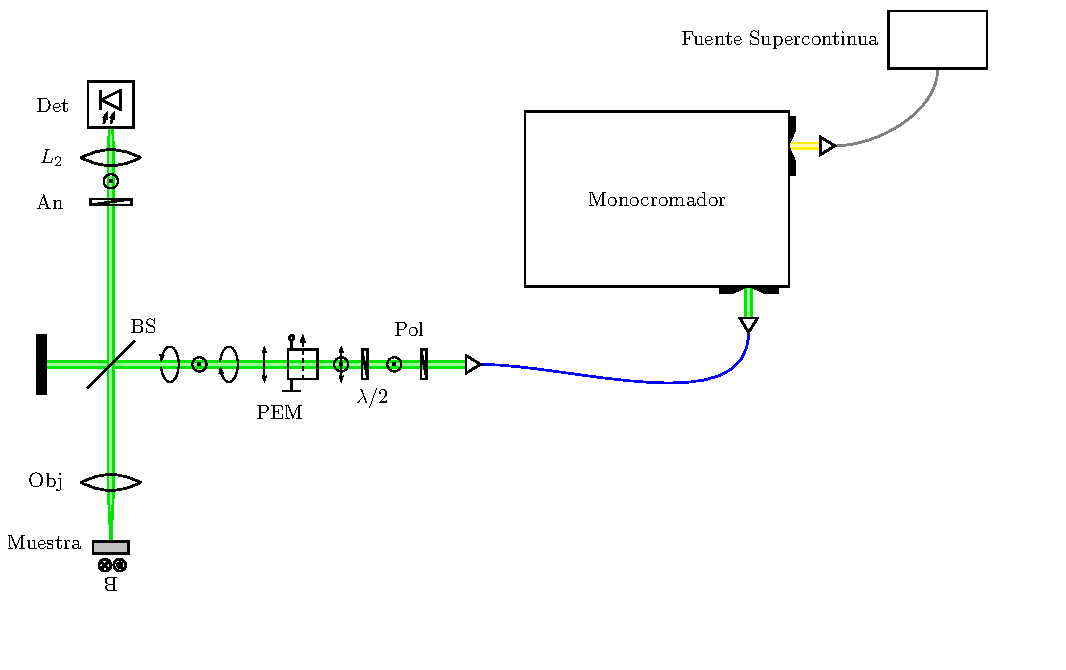
\includegraphics[scale=0.5]{figMet/diagrama/diagrama.pdf}
		\caption{Montaje Experimental}
	\end{figure}
	
}
\subsubsection{Programas de control}
\frame{
	\frametitle{Programa para adquirir la hist\'eresis}
	\begin{figure}[!hbt]
		\centering
		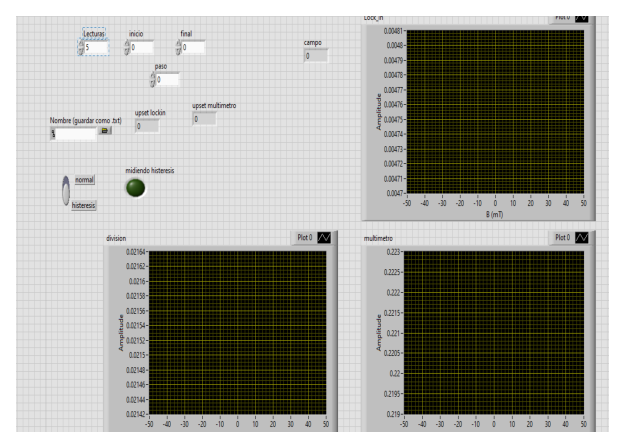
\epsfig{file=fiApLB/mk.eps, scale=0.7}
		\caption[Interfaz gr\'afica del software utilizado para obtener la hist\'eresis.]{Software para obtener la hist\'eresis. }
		\label{Lab:fig:mk}
	\end{figure}
}
\frame{
	\frametitle{Programa para adquirir espectro}
	\begin{figure}[!hbt]
		\centering
		\subfigure[Configuraci\'on]{
			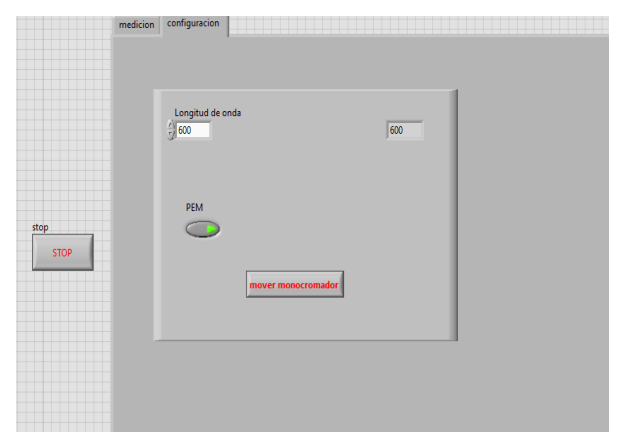
\epsfig{file=fiApLB/confEsp.eps, scale=0.4}
			\label{Lab:fig:conf}
		}
		\subfigure[Medici\'on]{
			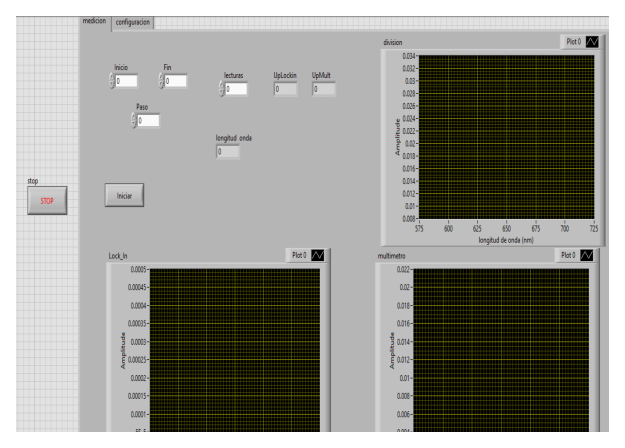
\epsfig{file=fiApLB/medEsp.eps, scale=0.4}
			\label{Lab:fig:med}
		}
		\caption[Interfaz gr\'afica del software utilizado para obtener el espectro de efecto Kerr.]{Software para obtener el espectro de efecto Kerr.}
		\label{Lab:fig:esp}
	\end{figure}
}
\endinput